%% LyX 1.3 created this file.  For more info, see http://www.lyx.org/.
%% Do not edit unless you really know what you are doing.
\documentclass[oneside,english]{book}
\usepackage[T1]{fontenc}
\usepackage[latin1]{inputenc}
\setcounter{secnumdepth}{3}
\setcounter{tocdepth}{3}
\usepackage{graphicx}
\usepackage{ae,aecompl}
\IfFileExists{url.sty}{\usepackage{url}}
                      {\newcommand{\url}{\texttt}}

\makeatletter
\usepackage{babel}
\makeatother
\begin{document}

\chapter{Using the GPS tools}


\section{What is GPS?}

GPS, the Global Positioning System, is a satellite-based system that
allows anyone with a GPS receiver to find their exact position anywhere
in the world. It is used as an aid in navigation, for example in airplanes,
in boats, and by hikers. The GPS receiver uses the signals from the
satellites to calculate its latitude, longitude and (sometimes) elevation.
Most receivers also have the capability to store locations (known
as \emph{waypoints}), sequences of locations that make up a planned
\emph{route}, and a tracklog or \emph{track} of the receivers movement
over time. Waypoints, routes, and tracks are the three basic feature
types in GPS data. QGIS displays waypoints in point layers while routes
and tracks are displayed in linestring layers.


\section{Loading GPS data from a file}

There are dozens of different file formats for storing GPS data. The
format that QGIS uses is called GPX (GPS eXchange format), which is
a standard interchange format that can contain any number of waypoints,
routes, and tracks in the same file.

\includegraphics{images/icon}To load a GPX file you need to use the \emph{GPS Tools} plugin. When
this plugin is loaded a button with a small handheld GPS device will
show up in the toolbar (the device looks a bit like a mobile phone).
Clicking on this button will open the \emph{GPS Tools} dialog (see
figure \ref{figure GPX loader}).

%
\begin{figure}

\caption{\label{figure GPX loader}The \emph{GPS Tools} dialog window}

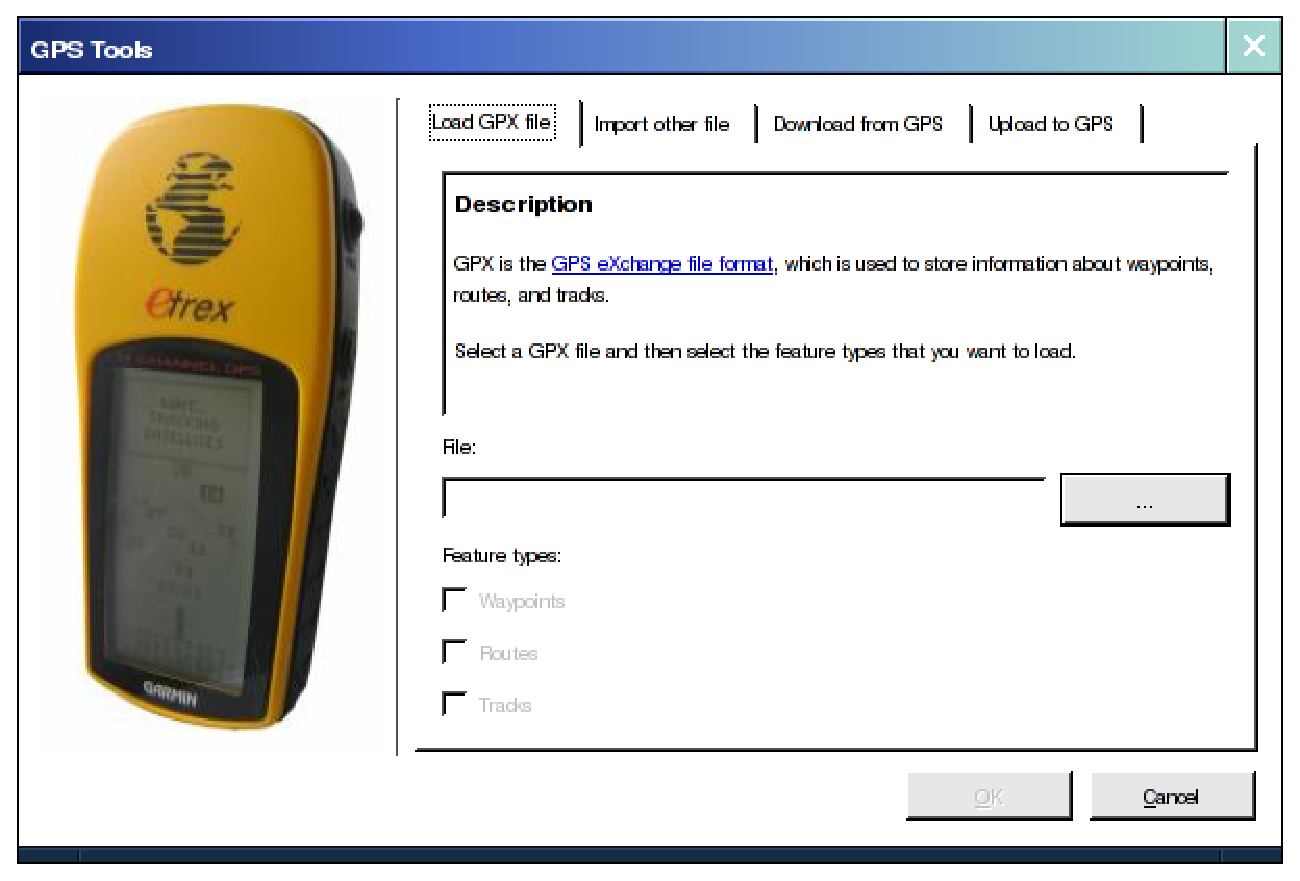
\includegraphics[%
  scale=0.5]{images/loadgpx}
\end{figure}


Use the browse button {[}...{]} to select the GPX file, then use the
checkboxes to select the feature types you want to load from that
GPX file. Each feature type will be loaded in a separate layer when
you click OK.


\section{GPSBabel}

Since QGIS uses GPX files you need a way to convert other GPS file
formats to GPX. This can be done for many formats using the free program
GPSBabel, which is available at \url{http://www.gpsbabel.org}. This
program can also transfer GPS data between your computer and a GPS
device. QGIS uses GPSBabel to do these things, so it is recommended
that you install it. However, if you just want to load GPS data from
GPX files you will not need it. Version 1.2.3 of GPSBabel is known
to work with QGIS, but you should be able to use later versions without
any problems.


\section{Importing GPS data}

To import GPS data from a file that is not a GPX file, you use the
tool \emph{Import other file} in the \emph{GPS Tools} dialog. Here
you select the file that you want to import, which featuretype you
want to import from it, where you want to store the converted GPX
file, and what the name of the new layer should be.

When you select the file to import you must also select the format
of that file by using the menu in the file selection dialog (see figure
\ref{figure importdialog}). All formats do not support all three
feature types, so for many formats you will only be able to choose
between one or two types.

%
\begin{figure}

\caption{\label{figure importdialog}File selection dialog for the import
tool}

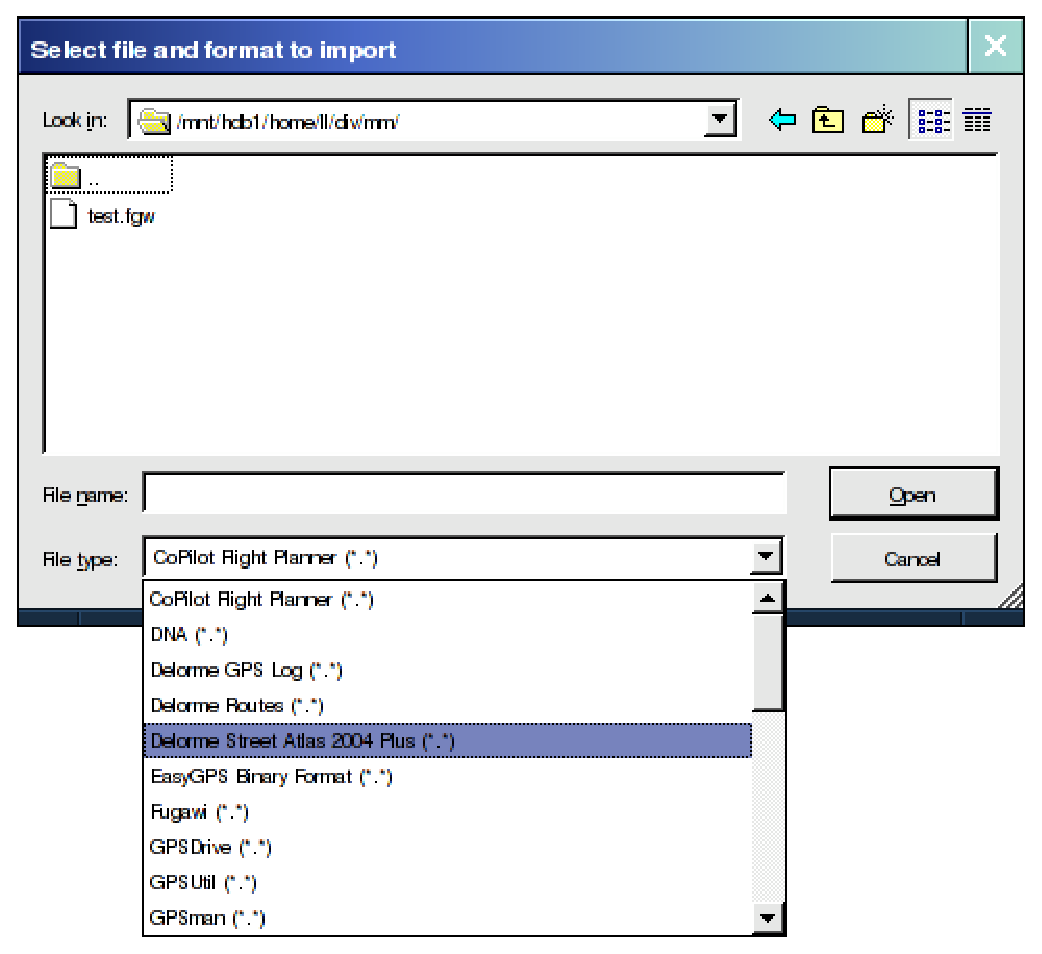
\includegraphics{images/importdialog}
\end{figure}



\section{Downloading GPS data from a device}

QGIS can use GPSBabel to download data from a GPS device directly
into vector layers. For this you use the tool \emph{Download from
GPS} (see figure \ref{figure download}), where you select your type
of GPS device, the port that it is connected to, the feature type
that you want to download, the GPX file where the data should be stored,
and the name of the new layer.

%
\begin{figure}

\caption{\label{figure download}The download tool}

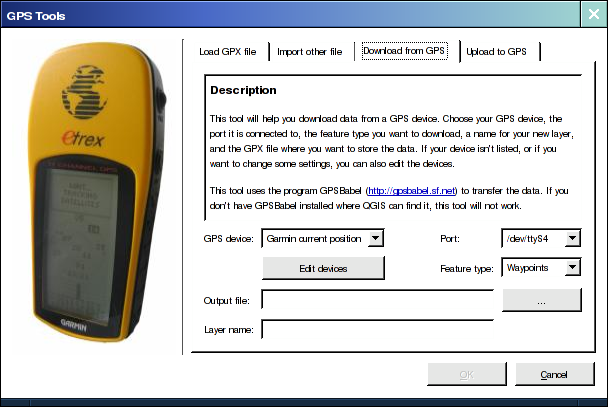
\includegraphics[%
  scale=0.5]{images/download}
\end{figure}


The device type you select in the GPS device menu determines how GPSBabel
tries to communicate with the device. If none of the device types
works with your GPS device you can create a new type (see section
\ref{sec:Defining-new-device}).

The port is a filename or some other name that your operating system
uses as a reference to the physical port in your computer that the
GPS device is connected to. On Linux this is something like /dev/ttyS0
or /dev/ttyS1 and on Windows it's COM1 or COM2.

When you click OK the data will be downloaded from the device and
appear as a layer in QGIS.


\section{Uploading GPS data to a device}

You can also upload data directly from a vector layer in QGIS to a
GPS device, using the tool \emph{Upload to GPS}. The layer must be
a GPX layer. To do this you simply select the layer that you want
to upload, the type of your GPS device, and the port that it's connected
to. Just as with the download tool you can specify new device types
if your device isn't in the list.

This tool is very useful together with the vector editing capabilities
of QGIS. You can load a map, create some waypoints and routes, and
then upload them and use them in your GPS device.


\section{\label{sec:Defining-new-device}Defining new device types}

There are lots of different types of GPS devices. The QGIS developers
can't test all of them, so if you have one that does not work with
any of the device types listed in the download and upload tools you
can define your own device type for it. You do this by using the \emph{GPS
device editor}, which you start by clicking the \emph{Edit devices}
button in the download or the upload window.

To define a new device you simply click the \emph{New device} button,
enter a name, a download command, and an upload command for your device,
and click the \emph{Update device} button. 

The name will be listed in the device menus in the upload and download
windows, and can be any string. 

The download command is the command that is used to download data
from the device to a GPX file. This will probably be a GPSBabel command,
but you can use any other command line program that can create a GPX
file. QGIS will replace the keywords \emph{\%type}, \emph{\%in}, and
\emph{\%out} when it runs the command.

\emph{\%type} will be replaced by {}``-w'' if you are downloading
waypoints, {}``-r'' if you are downloading routes, and {}``-t''
if you are downloading tracks. These are command line options that
tell GPSBabel which feature type to download. 

\emph{\%in} will be replaced by the port name that you choose in the
download window, and \emph{\%out} will be replaced by the name you
choose for the GPX file that the downloaded data should be stored
in. So if you create a device type with the download command {}``gpsbabel
\%type -i garmin -o gpx \%in \%out'' (this is actually the download
command for the predefined device type {}``Garmin serial'') and
then use it to download waypoints from port {}``/dev/ttyS0'' to
the file {}``output.gpx'', QGIS will replace the keywords and run
the command {}``gpsbabel -w -i garmin -o gpx /dev/ttyS0 output.gpx''.

The upload command is the command that is used to upload data to the
device. The same keywords are used, but \emph{\%in} is now replaced
by the name of the GPX file for the layer that is being uploaded,
and \emph{\%out} is replaced by the port name. You can learn more
about GPSBabel and it's available command line options at \url{http://www.gpsbabel.org}

Once you have created a new device type it will appear in the device
lists for the download and upload tools.
\end{document}
